\input ../SlidePreamble
\input ../preamble


\begin{document}

{\Huge


\centerline{\bf TTIC 31230, Fundamentals of Deep Learning}
\bigskip
\centerline{David McAllester, April 2017}

\vfill
\centerline{\bf Over-Fitting and Regularization}
\vfill
\vfill

\centerline{}
\slide{Over Fitting}

If we have more parameters than data then we can fit any set of labels.

\vfill
\begin{quotation}
``Our experiments establish that state-of-the-art convolutional networks
for image classification trained with stochastic gradient methods easily fit a random
labeling of the training data.''
\end{quotation}

\vfill
\rightline{Rethinking Generalization, Zhang et al., ICLR 2017}


\slide{Train Data, Development Data and Test Data}

Data is typically divided into {\bf a training set}, {\bf a development set} and {\bf a test set} each drawn IID from the population.

\vfill
A learning algorithm optimizes training loss.

\vfill
One then optimizes algorithm design (and hyper-parameters) on the development set. (graduate student descent).

\vfill
Ultimate performance should be done on a test set not used for development.  Test data is often withheld from developers.

\slideplain{Loss Vs. Error Rate}
While training (gradient descent) is generally done on cross entropy loss, performance is often judged by other measures such as classification error rate.

\vfill
The term ``loss'' is often used as a synonym for cross entropy loss.

\vfill
Hence one often reports both ``loss'' and ``error rate''.

\vfill
Note that classification error rate is not differentiable.


\slide{Early Stopping}

\centerline{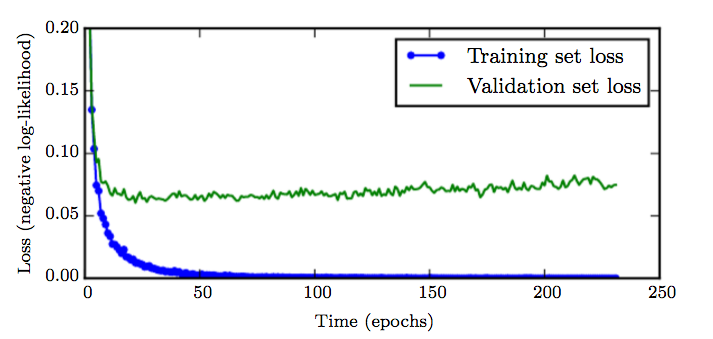
\includegraphics[width = 6in]{../images/EarlyStopping}}

\centerline{\huge [Goodfellow et al.]}

\vfill
During SGD one should be tracking validation loss.

\vfill
A typical rule is to stop when the validation loss has not set a new record low for some period.

\ignore{
  The following slide is not true --- gradient flow approaches the optimum directly along the smallest eigenvector of H.  The regularization path
  satisfies g = lambda(t) Phi and approaches with a fixed nonzero angle to the eigenvector.
  
\slide{Early Stopping}

\centerline{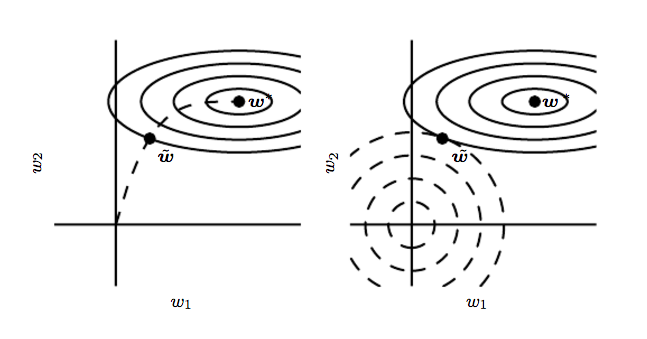
\includegraphics[width = 7in]{../images/EarlyStopping2}}
\centerline{[Goodfellow et al.]}

\vfill
For differential Newton updates (gradient flow) on a quadratic loss function, with $\Phi$ initialized to zero, early stopping and $L_2$ regularization are equivalent.
}

\slide{Early stopping on Random Labels}

\centerline{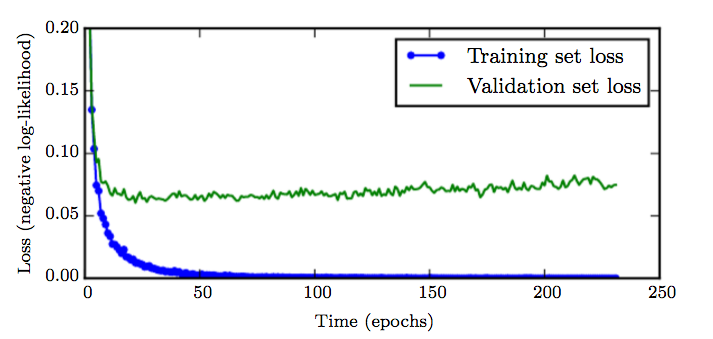
\includegraphics[width = 6in]{../images/EarlyStopping}}

\centerline{\huge [Goodfellow et al.]}


\vfill
For random labels the optimal score function is the constant zero which, for binary classification, has a loss of $\ln 2 \approx .69$.

\vfill
If the validation data is random then the validation loss should start to climb immediately.

\ignore{
\slide{Hinton vs. Chomsky}

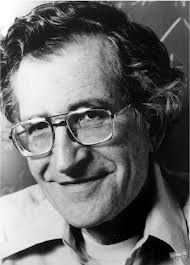
\includegraphics[width=1.0 in]{../images/Chomsky} \begin{minipage}[b]{8in} Noam Chomsky: 
Natural language grammar is unlearnable without with an innate linguistic capacity. This position is supported by the ``no free lunch theorem''.\end{minipage}

\vfill
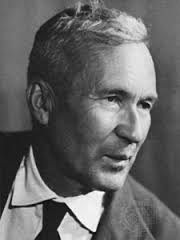
\includegraphics[height=1.0 in]{../images/Kolmogorov}
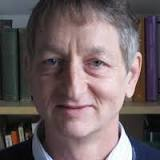
\includegraphics[height=1.0 in]{../images/Hinton}
\begin{minipage}[b]{7in}
Andrey Kolmogorov, Geoff Hinton: Universal learning algorithms exist. This position is supported by the ``free lunch theorem''.
\end{minipage}

\slide{The No Free Lunch Theorem}

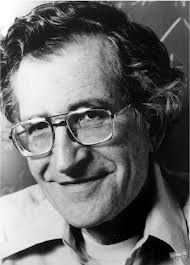
\includegraphics[width=1.0 in]{../images/Chomsky} 

Without prior knowledge, such as universal grammar, it is impossible to make a prediction for an input you have not seen in the training data.


\vfill
{\bf Proof:} Select a predictor $h$ uniformly at random from all functions from ${\cal X}$ to ${\cal Y}$ and then take the data distribution to draw pairs $(x, h(x))$
where $x$ is drawn uniformly from ${\cal X}$.  No learning algorithm can predict $h(x)$ where $x$ does not occur in the training data.

}

\slide{PAC-Bayesian Generalization Guarantees}

It is possible to prove formal generalization guarantees without looking at the validation or test data.

\vfill
To do this we assume a prior distribution on models.

\vfill
Intuitively, for any prior (true or not) selected before seeing the data, one can prove that
any model with high posterior probability must generalize well.

\vfill
But there is no guarantee that any model will have sufficiently large posterior probability.


\slide{PAC-Bayesian Generalization Guarantees}

Consider an arbitrary prior probability distribution over an arbitrary discrete class ${\cal H}$ of ``hypotheses'' (or models).

\vfill
Consider a population distribution over pairs $(x,y)$ with $x \in {\cal X}$ and $y \in {\cal Y}$.

\vfill
Consider a loss function ${\cal L}(h,x,y)$ such that for any $h \in {\cal H}$ and pair $(x,y)$ we have
${\cal L}(h,x,y) \in (0,L_\mathrm{max})$.

\vfill
For example ${\cal }(h,x,y) = \min(L_\mathrm{max},\; - \ln\; P(y|h,x))$.

\slide{PAC-Bayesian Generalization Guarantees}
\begin{eqnarray*}
{\cal L}(h)  & = &  E_{(x,y)\sim \mathrm{Pop}}\;{\cal L}(h,x,y) \\
\\
\hat{{\cal L}}(h) & = & E_{(x,y)\sim \mathrm{Train}}\;{\cal L}(h,x,y)
\end{eqnarray*}

\vfill
    {\bf Theorem:} With probability
    at least $1-\delta$ over an I.I.D. draw of training data from the population the following holds {\em simultaneously} for all $h \in {\cal H}$.

\vfill
    $${\cal L}(h) \leq \frac{10}{9}\parens{\hat{\cal L}(h) + \frac{5 L_\mathrm{max}}{N}\parens{\ln\frac{1}{P(h)} + \ln\frac{1}{\delta}}}$$

\slide{A Model Compression Guarantee}

Let $|\Phi|$ be the number of bits used to represent $\Phi$ under some fixed compression scheme.

\vfill
Let $P(\Phi) = 2^{-|\Phi|}$

\vfill
    $${\cal L}(\Phi) \leq \frac{10}{9}\parens{\hat{\cal L}(\Phi) + \frac{5 L_\mathrm{max}}{N}\parens{(\ln 2)|\Phi| + \ln\frac{1}{\delta}}}$$

\slide{A Weight Norm Guarantee}

\vfill
\begin{eqnarray*}
P(w) & = & {\cal N}(0,\sigma)^d \\
  \\
L(\Theta) & = & \expectsub{\epsilon \sim {\cal N}(0,\sigma)^d}{{\cal L}(\Theta+\epsilon)} \\
\\
\hat{L}(\Theta) & = & \expectsub{\epsilon \sim {\cal N}(0,\sigma)^d}{\hat{{\cal L}}(\Theta+\epsilon)}
\end{eqnarray*}

\vfill
\begin{eqnarray*}
   L(\Theta) & \leq & \frac{10}{9}\parens{\hat{L}(\Theta) + \frac{5 \lmax}{N}\parens{\frac{||\Theta||^2}{2\sigma^2} + \ln \frac{1}{\delta}}}
\end{eqnarray*}

\slide{$L_2$ Regularization (a.k.a. Weight Decay or Shrinkage)}

$$\Phi^* = \argmin_\Phi \;E_{(x,y) \sim \mathrm{Train}}\;{\cal L}(\Phi,x,y) + \frac{1}{2}\lambda||\Phi||^2$$

\vfill
\begin{eqnarray*}
  & & \nabla_\Phi \;\left(E_{(x,y) \sim \mathrm{Batch}}\;{\cal L}(\Phi,x,y) + \frac{1}{2}\lambda||\Phi||^2\right) \\
  \\
  & = & g(\Phi) + \lambda \Phi \;\;\;\mbox{giving }\;{\color{red} \Phi^* = \frac{g(\Phi^*)}{\lambda}} \\
  \\
  \Phi_{t+1} & = & {\color{red} \Phi_t - \eta \hat{g}_t - \eta \lambda \Phi_t}
\end{eqnarray*}

\slide{Standard Parameterization}

The update
$$\Phi_{t+1} = \Phi_t - \eta \hat{g}_t - \eta \lambda \Phi_t$$

\vfill
is typically parameterized as
$$\Phi_{t+1} = \Phi_t - \eta \hat{g}_t - \gamma \Phi_t$$
where $\gamma$ is the weight decay parameter.

\vfill
{\color{red} However, the $\eta$, $\lambda$ parameterization may be less ``entangled'' in hyper-parameter search than the $\eta$, $\gamma$ parameterization.}

\slide{The Gradient Smoothing Parameterization}

Setting $\eta = \gamma/\lambda$ we get

\begin{eqnarray*}
  \Phi_{t+1} & = & \Phi_t - \frac{\gamma}{\lambda} \hat{g}_t - \gamma \Phi_t \\
  \\
  & = & \left(1 -\gamma\right)\Phi_t - \gamma\left(\frac{\hat{g}_t}{\lambda}\right) \\
  \\
  \Phi^* & = & \frac{g}{\lambda}
\end{eqnarray*}

\vfill
Again, different parameterizations will have different degrees of entanglement between the parameters
and reflect different semantic interpretations.

\slide{Shrinkage meets Early Stopping}

Early stopping can limit $||\Phi||$ --- growing a large $||\Phi||$ can take a long time.

\vfill
Early stopping seems more related to limiting $||\Phi - \Phi_\mathrm{init}||$
\vfill

Theoretical guarantees work for $||\Phi - \Phi_{\mathrm{init}}||^2$ just as well as for $||\Phi||^2$.

\vfill
This suggests replacing $L_2$ regularization with

\vfill
$$\Phi^* = \argmin_\Phi {\cal L}(\Phi) + \frac{1}{2}\lambda ||\Phi- \Phi_{\mathrm{init}}||^2$$

\slide{Shrinkage meets Batch Scaling}

We have some in-house evidence that shinkage is important in batch scaling.

\vfill
Batch scaling with shrikage seems better behaved than batch scaling without shrikage.

\vfill
\centerline{?????}

\slide{$L_1$ Regularization and Sparse Weights}

$$p(\Phi) \propto e^{-||\Phi||_1} \;\;\;\;\;\;\;\;||\Phi||_1 = \sum_i |\Phi_i|$$

$$\Phi^* = \argmin_\Phi \; \;\;\hat{\cal L}(\Phi) \;+ \; \;\lambda||\Phi||_1$$

\begin{eqnarray*}
  \Phi & \minuseq & \eta \nabla_\Phi \; \ell_{\mathrm{train}}(\Phi) \\
  \Phi_i & \minuseq & \eta\lambda\; \mathrm{sign}(\Phi_i) \;\;\;\;\;\;\mbox{(shrinkage)}
\end{eqnarray*}

\vfill
At equilibrium \hfill (sparsity is difficult to achieve with SGD)

$$\begin{array}{rcll}
\Phi_i &  = & 0  & \;\;\;\;\;\mbox{if} \;\left|\partial \ell /\partial \Phi_i\right| <  \lambda \\
\partial \ell /\partial \Phi_i & = &  -\lambda \mathrm{sign}(\Phi_i) &\;\;\;\;\; \mbox{otherwise}
\end{array}$$


\slide{Ensembles}

Train several models $\mathrm{Ens} = (\Phi_1,\;\ldots,\; \Phi_k)$ from different initializations and/or under different meta parameters.

\vfill
We define the ensemble model by
$$P_\mathrm{Ens}(y|x) = \frac{1}{k} \sum_{j=1}^k\; P_{\Phi_i}(y|x)$$

\vfill
Ensemble models almost always perform better than any single model.

\vfill
We will explore some reasons for this.


\vfill
\slide{Ensembles Under Cross Entropy Loss}

For log loss we average the probability vectors.

\vfill
$$P(y|x) = \frac{1}{k} \sum_i \;P_i(y|x)$$

\vfill
$- \log P$ is a convex function of $P$.  For any convex $\ell(P)$ Jensen's inequality states that

$$\ell\left(\frac{1}{k} \sum_i P_i\right) \leq \frac{1}{k} \sum_i \ell(P_i)$$

\vfill
This implies that the loss of the average model cannot be worse (can only be better) than the average loss of the models.


\ignore{
\slide{Ensembles under Square Loss}

We average $k$ regression models

\vfill
\begin{eqnarray*}
  f(x) & = & \frac{1}{k} \sum_{i=1}^k\; f_i(x) \\
  \\
  \\
  f(x) - y & = & \frac{1}{k} \sum_{i=1}^k\; (f_i(x) - y) \\
  \\
  \\
  \epsilon & = & \frac{1}{k}  \sum_{i=1}^k\; \epsilon_i,\;\;\epsilon_i = f_i - y \;\;\;\mbox{(residuals)}
\end{eqnarray*}



\slide{Ensembles for Square Loss}

Assume that $\expect{\epsilon_i ^2} = \sigma^2$ and $\expect{\epsilon_i \epsilon_j} = \sigma^2\rho$ for $i \not = j$.

\begin{eqnarray*}
  \expect{\left(\frac{1}{k} \sum_i \epsilon_i\right)^2} & = & \frac{1}{k^2} \expect{\sum_i\;\left(\epsilon_i^2 + \sum_{j \not = i}\;\epsilon_i\epsilon_j\right)} \\
  \\
  \\
  & = & \frac{1}{k} \sigma^2 + \frac{k-1}{k} \sigma^2\rho \;=\; \sigma^2\left(\frac{1}{k} + \left(1-\frac{1}{k}\right)\rho\right)
\end{eqnarray*}

\vfill
If Pearson's correlation $\rho = \expect{\epsilon_i\epsilon_j}/\sigma^2 < 1$ we win.
}


\slide{Implicit Regularization}

Any stochastic learning algorithm, such as SGD, determines a stochastic mapping from training data to models.

\vfill
The algorithm can implicitly incorporate a preference or bias for models.

\vfill
For example, solving linear least squares regression with SGD maintains the invariant that $\Phi$ is a linear combination of training vectors.

\vfill
It is not hard to show that SGD finds the zero training error solution minimizing $||\Phi||$.

\vfill
So solving least squares regression by SGD has an implicit weight norm regularization.

\slideplain{An Implicit Regularization Generalization Guarantee}

let $A(\mathrm{Train})$ be the distribution on models defined by running the stochastic algorithm $A$ on training data
$\mathrm{Train}$.

\vfill
We let $\overline{A}$ be the distribution on models defined first drawing $\mathrm{Train}$ and then drawing a model from $A(\mathrm{Train})$.

\begin{eqnarray*}
\overline{A}(\Phi) & = & E_{\mathrm{Train} \sim \mathrm{Pop}}\;A(\mathrm{Train})(\Phi) \\
\\
L_A(\mathrm{Train}) & = & E_{\Phi \sim A(\mathrm{Train})};E_{(x,y) \sim \mathrm{Pop}}\;{\cal L}(\Phi,x,y) \\
\\
\hat{L}_A(\mathrm{Train}) & = & E_{\Phi \sim A(\mathrm{Train})}\;E_{(x,y) \sim \mathrm{\mathrm{Train}}}\;{\cal L}(\Phi,x,y)
\end{eqnarray*}

\ignore{
\slide{Optimality of $Q_{\cal A}(\mathrm{Pop})$}

Consider an arbitrary prior $P$.

\vfill
\begin{eqnarray*}
  & & E_{\mathrm{Train}\sim\mathrm{Pop}}\;KL(Q_{\cal A}(\mathrm{Train}),P) \\
  \\
  & = & E_{\mathrm{Train}\sim\mathrm{Pop}}\;\ln \frac{Q_{\cal A}(\mathrm{Train})(h)}{P(h)}  \\
\\
\\
& = & \expectsub{\mathrm{Train}\sim \mathrm{Pop},\;h \sim Q_{\cal A}(\mathrm{Train})}{\ln \frac{Q_{\cal A}(\mathrm{Train})(h)}{Q_{\cal A}(\mathrm{Pop})(h)}} \\
\\
\\
& & + \expectsub{h \sim Q_{\cal A}(\mathrm{Pop})}{\ln \frac{Q_{\cal A}(\mathrm{Pop}(h))}{P(h)}}
\end{eqnarray*}

\slideplain{Optimality of $Q_{\cal A}(\mathrm{Pop})$}

\begin{eqnarray*}
  & & E_{\mathrm{Train}\sim\mathrm{Pop}}\;KL(Q_{\cal A}(\mathrm{Train}),P) \\
\\
& = & \expectsub{\mathrm{Train}\sim \mathrm{Pop}}{KL(Q_{\cal A}(\mathrm{Train}),Q_{\cal A}(\mathrm{Pop}))} + KL(Q_{\cal A}(\mathrm{Pop}),P)
\end{eqnarray*}

\vfill
So $Q_{\cal A}(\mathrm{Pop})$ is an {\bf optimal prior} (or {\bf implicit prior}) for algorithm ${\cal A}$.
}

\slide{An Implicit Regularization Generalization Guarantee}

For any given learning algorithm ${\cal A}$ and we have the following with probability at least $1-\delta$ over the draw of $\mathrm{Train}$.

\vfill
$$L(\mathrm{Train}) \leq \frac{10}{9}\parens{\hat{L}(\mathrm{Train}) + \frac{5\lmax}{N}\parens{KL(A(\mathrm{Train}),\;\overline{A}) + \ln \frac{1}{\delta}}}$$

\ignore{
\slide{The Broad Basin Hypothesis}

Do broad basins in the loss function generalize better?

\vfill

{\bf Flat Minima:} Hochreiter and Schmidhuber (1997)

\vfill
{\bf On Large-Batch Training for Deep Learning: Generalization Gap and Sharp Minima:} Keskar et al. (Nocedal) arXiv 2016, ICLR 2017.

\vfill
{\bf Sharp Minima Can Generalize For Deep Nets:} Dihn et al. (both Bengios) arXiv 2017.

\vfill
I believe that the PAC-Bayesian analysis supports the broad basin hypothesis.  We are interested in the implicit prior (implicit geometry) of SGD
and ``broad'' should be defined in terms of that geometry.
}

\ignore{
\slide{Sparse Activation}

We can impose an $L_1$ regularization on the activations of the network (the output of the activation function of each neuron).

$$\Phi^* = \argmin_\Phi \ell(\Phi) + \lambda||h||_1$$

\vfill
where $h$ is the vector of neuron activation outputs.

\vfill
This will tend to make activations sparse.

\slide{Sparse Coding}

Let $W$ be a matrix where we view $W_{\cdot,i}$ is the $i$th ``dictionary vector''.

\vfill
For input $x$ we can construct a $k$-sparse representation $h(x)$.

\vfill
$$h(x) = \argmin_{h,||h||_0=k} \;||x - Wh||^2$$

\vfill
Note

$$Wh = \sum_{i \in I(x)} \; h_i \; W_{\cdot,i}\;\;\;\;\;|I(x)| = k$$

\vfill
We can now replace $x$ by its sparse code $h(x)$.

}

\ignore{
\slide{Modeling the Implicit Prior}

We divide the parameters into classes where we write $c_i$ for the class of parameter $w_i$.

\vfill
We let $w_i^0$ be the initial value of $w_i$ and let $w_i^f(S)$ be the final value of $w_i$.

\vfill
\begin{eqnarray*}
\beta_{c,1},\beta_{c,2} & = & E_{S \sim D^N}\;\argmin_{\beta_1,\beta_2}\; \sum_{i: c_i = c}\;(w_i^f(S) - (\beta_1 w_i^0 + \beta_2))^2 \\
\beta_{c,3},\beta_{c,4} &  = & E_{S \sim D^N}\; \argmin_{\beta_3,\beta_4}\;\sum_{i: c_i = c}\;((w_i^f(S) - (\beta_{c_1,1} w_i^0 + \beta_{c_i,2}))^2 - (\beta_3 w_i^0 + \beta_4))^2
\end{eqnarray*}

We then consider the prior distribution $P$ on $w_i$ to be a Gaussian with mean $\mu_i$ and standard deviation $\sigma_i$ given by

\begin{eqnarray*}
  \mu_i & = & \beta_{c_i,1}w_i^0 + \beta_{c_i,2} \\
  \sigma_i^2 & = & \beta_{c_i,3}w_i^0 + \beta_{c_i,4}
\end{eqnarray*}

\slide{Modeling the Implicit Prior}

This prior does not depend on any particular training data $S$ and hence is a legitimate prior.

\vfill
In practice we can estimate this prior from the training data.

\begin{eqnarray*}
\hat{\beta}_{c,1},\hat{\beta}_{c,2} & = & \argmin_{\beta_1,\beta_2} \sum_{i: c_i = c}\;(w_i^f(S) - (\beta_1 w_i^0 + \beta_2))^2 \\
\hat{\beta}_{c,3},\hat{\beta}_{c,4} &  = & \argmin_{\beta_3,\beta_4} \sum_{i: c_i = c}\;((w_i^f(S) - (\hat{\beta}_{c_i,1} w_i^0 + \hat{\beta}_{c_i,2}))^2 - (\beta_3 w_i^0 + \beta_4))^2
\end{eqnarray*}
}

\slide{Dropout}

Dropout can be viewed as an ensemble method.


\vfill
To draw a model from the ensemble we randomly select a mask $\mu$ with

$$\left\{\begin{array}{ll} \mu_i = 0 & \mbox{with probability $\alpha$} \\ \\ \mu_i = 1 & \mbox{with probability $1-\alpha$}
\end{array}\right.$$

\vfill
Then we use the model $(\Phi,\;\mu)$ with weight layers defined by


\vfill
$$y_i = \mathrm{Relu}\left(\sum_j\;W_{i,j} \;\mu_jx_j\right)$$

\slide{A Dropout Bound}

\begin{eqnarray*}
KL(Q_{\alpha,\Phi},\;Q_{\alpha,0}) & = & \expectsub{\mu \sim P_\alpha, \epsilon \sim {\cal N}(0,1)^d}
{\ln \frac{P_\alpha(\mu) e^{-\frac{1}{2}||\mu \odot \epsilon||^2}}{P_\alpha(\mu) e^{-\frac{1}{2}||\mu \odot (\Phi + \epsilon)||^2}}} \\
\\
& = & \expectsub{\mu \sim P_\alpha}{\frac{1}{2}||\mu \odot \Phi||^2} \\
\\
& = & \frac{1-\alpha}{2}||\Phi||^2
\end{eqnarray*}

$$L(Q_{\alpha,\Phi}) \leq \frac{1}{1-\frac{1}{2\lambda}}\parens{\hat{L}(Q_{\alpha,\Phi}) + \frac{\lambda \lmax}{N}\parens{\frac{1-\alpha}{2}||\Phi||^2 + \ln \frac{1}{\delta}}}$$

\slide{Dropout Training}

Repeat:

\vfill

\begin{itemize}
\item Select a random dropout mask $\mu$
  
\vfill
\item $\Phi \;\minuseq\; \nabla_\Phi\; \ell(\Phi, \mu)$
\end{itemize}

\vfill
Backpropagation must use the same mask $\mu$ used in the forward computation.

\slide{Test Time Scaling}


\vfill
At train time we have

\vfill
$$y_i = \mathrm{Relu}\left(\sum_j\;W_{i,j} \;\mu_j x_j\right)$$


\vfill
At test time we have

\vfill
$$y_i = \mathrm{Relu}\left((1-\alpha)\;\sum_j\;W_{i,j} \;x_j\right)$$

\vfill
At test time we use the ``average network''.

\slide{Dropout for Least Squares Regression}

Consider simple least square regression

\begin{eqnarray*}
  \Phi^* & = &  \argmin_\Phi\;\; \mathrm{E}_{(x,y)} \;\expectsub{\mu}{(y - \Phi \cdot (\mu \odot x))^2} \\
  \\
  & = & \expect{(\mu\odot x)(\mu\odot x)^{\top}}^{-1}\; \expect{y (\mu\odot x)} \\
  \\
  & = & \argmin_\Phi\;\; \mathrm{E}_{(x,y)} (y - (1-\alpha) \Phi \cdot x)^2 + \sum_i\frac{1}{2}(\alpha - \alpha^2) \expect{x_i^2} \Phi_i^2
\end{eqnarray*}

\vfill
In this case dropout is equivalent to a form of $L_2$ regularization --- see Wager et al. (2013).

\slide{Proof of the Discrete PAC-Bayes Bound}
$${\cal L}(h) = E_{(x,y)\sim \mathrm{Pop}}\;{\cal {\cal L}}(h,x,y)$$

\vfill
$$\hat{{\cal L}}(h) = E_{(x,y)\sim \mathrm{Train}}\;{\cal {\cal L}}(h,x,y)$$

\slide{Proof}

Consider $\lmax = 1$ and define $\epsilon(h)$ by

\vfill
$$\epsilon(h) = \sqrt{\frac{2{\cal L}(h)\parens{\ln\frac{1}{P(h)} + \ln\frac{1}{\delta}}}{N}}.$$

\vfill
By the relative Chernoof bound we have

\vfill
$$P_{\mathrm{Train} \sim \mathrm{Pop}}\parens{\hat{{\cal L}}(h) \leq {\cal L}(h) - \epsilon(h)} \leq e^{-N\frac{\epsilon(h)^2}{2{\cal L}(h)}} = \delta P(h).$$

\slide{Proof}

$$P_{\mathrm{Train} \sim \mathrm{Pop}}\parens{\hat{{\cal L}}(h) \leq {\cal L}(h) - \epsilon(h)} \leq \delta P(h).$$

\vfill
$$P_{\mathrm{Train} \sim \mathrm{Pop}}\parens{\exists h\;\hat{{\cal L}}(h) \leq {\cal L}(h) - \epsilon(h)} \leq \sum_h \delta P(h) =\delta$$

\vfill
$$P_{\mathrm{Train} \sim \mathrm{Pop}}\parens{\forall h\;{\cal L}(h) \leq \hat{{\cal L}}(h) + \epsilon(h)} \geq 1- \delta$$

\slide{Proof}

$${\cal L}(h) \leq \widehat{{\cal L}}(h) + \sqrt{{\cal L}(h)\parens{\frac{2\parens{\ln\frac{1}{P(h)} + \ln\frac{1}{\delta}}}{N}}}$$

using
$$\sqrt{ab} = \inf_{\lambda > 0}\;\frac{a}{2\lambda} + \frac{\lambda b}{2}$$
\vfill
we get
$${\cal L}(h) \leq \widehat{{\cal L}}(h) + \frac{{\cal L}(h)}{2\lambda} + \frac{\lambda\parens{\ln\frac{1}{P(h)} + \ln\frac{1}{\delta}}}{N}$$

\slide{Proof}
$${\cal L}(h) \leq \widehat{{\cal L}}(h) + \frac{{\cal L}(h)}{2\lambda} + \frac{\lambda\parens{\ln\frac{1}{P(h)} + \ln\frac{1}{\delta}}}{N}$$

\vfill
Solving for ${\cal L}(h)$ yields

\vfill
$${\cal L}(h) \leq \frac{1}{1-\frac{1}{2\lambda}}\parens{\hat{{\cal L}}(h) + \frac{\lambda}{N}\parens{\ln \frac{1}{P(h)} + \ln \frac{1}{\delta}}}$$

\vfill
Setting $\lambda = 5$ and rescaling the loss gives the version on earlier slides.

\ignore{
\slide{A KL Divergence Bound}

Let $P$ be any ``prior'' and $Q$ be any ``posterior'' on any model space.

\vfill
Define
\begin{eqnarray*}
  L(Q) & =  &\expectsub{h \sim Q}{L(h)} \\
  \\
  \hat{L}(Q) & =  &\expectsub{h \sim Q}{\hat{L}(h)}
\end{eqnarray*}


\vfill
For any $P$ and any $\lambda > \frac{1}{2}$, with probability
at least $1-\delta$ over the draw of the training data, the following holds simultaneously for all $Q$.
\vfill
$$L(Q) \leq \frac{1}{1-\frac{1}{2\lambda}}\parens{\hat{L}(Q) + \frac{\lambda \lmax}{N}\parens{KL(Q,P) + \ln \frac{1}{\delta}}}$$

\slide{$L_2$ PAC-Bayesian Bounds in Action}

Computing Nonvacuous Generalization Bounds for Deep (Stochastic) Neural Networks with Many More Parameters than Training Data, (Dziugaite and Roy, arXiv, 2017)

\vfill
\centerline{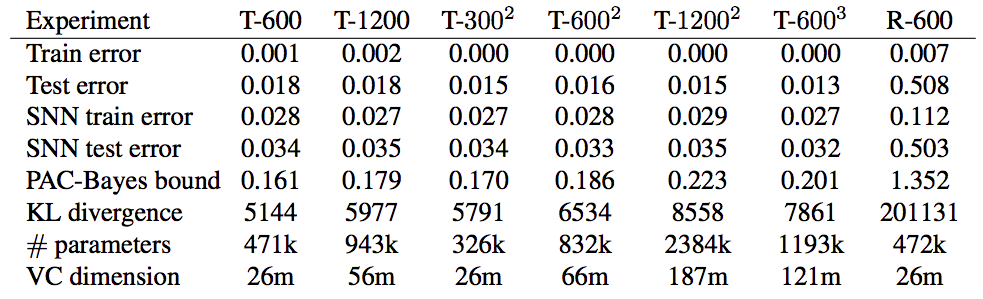
\includegraphics[width = 8in]{../images/Roy}}

\vfill
{\bf The bounds are based on $L_2$ distance of the weight vector to the initialization.}

\vfill
{\bf The weight vector is retrained to minimize the bound.}
}

\slide{END}

}
\end{document}

